Qui, di seguito, viene riportata l'architettura relativa alla seconda solution.

\lstinputlisting[language=C++]{solutions/s4/s4.cpp}

In particolare, nella soluzione hardware in questione, rispetto alla solution 1, è stata aggiunto la direttiva di unrolling con fattore pari a 2 all'interno del loop1.

\begin{figure}[H]
	\centering
	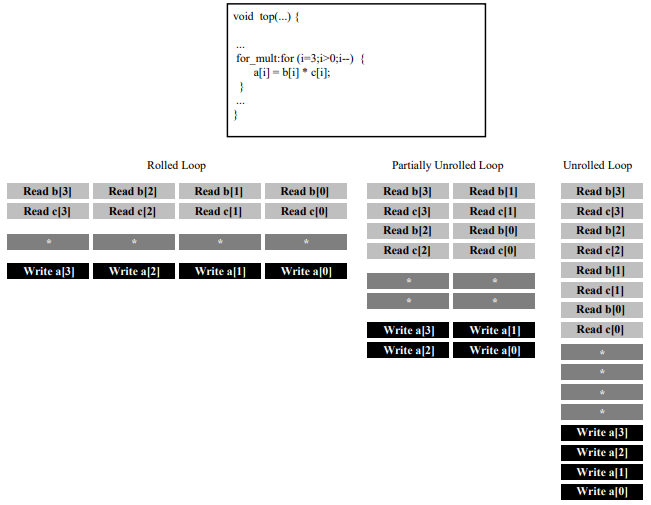
\includegraphics[width=0.5\textwidth]{solutions/s4/unrolling.png}
	\caption{HLS Loop Unrolling}
\end{figure}

Effettuando la sintesi è possibile evidenziare il seguente report:\\

\begin{table}[H]
	\centering
	\begin{minipage}[t]{0.45\linewidth}
		\centering
		\begin{tabular}{|c|c|c|c|}
			\hline
			\textbf{Clock} & \textbf{Target} & \textbf{Estimated} & \textbf{Uncertainty} \\
			\hline
			ap\_clk & 10.00 & 8.510 & 1.25 \\
			\hline
		\end{tabular}
		\caption{HLS Solution 4 Timing Summary (ns)}
		\label{tab:hls-solution-4-timing-summary}
	\end{minipage}
	\hfill
	\begin{minipage}[t]{0.45\linewidth}
		\centering
		\begin{tabular}{|c|c|c|c|}
			\hline
			\multicolumn{2}{|c|}{\textbf{Latency}} & \multicolumn{2}{|c|}{\textbf{Interval}} \\
			min & max & min & max \\
			\hline
			11 & 91 & 11 & 91 \\
			\hline
		\end{tabular}
		\caption{HLS Solution 4 Latency Summary (clock cycles)}
		\label{tab:hls-solution-4-latency-summary}
	\end{minipage}
\end{table}

In particolare, si può notare come il valore di trip count del loop1 risulta essere dimezzato rispetto alla solution 1. Questo è dovuto all'attuazione della direttiva  di unrolling di fattore 2 sul loop1 e così permettendo l'esecuzione in parallelo di due iterazioni.

\begin{table}[H]
	\centering
	\begin{tabular}{|c|c|c|c|c|c|c|c|c|}
		\hline
		\multicolumn{1}{|c|}{Loop} & \multicolumn{2}{|c|}{\textbf{Latency}} & \multicolumn{1}{c|}{\textbf{Iteration Latency}} & \multicolumn{2}{c|}{\textbf{Initiation Interval}} & \multicolumn{1}{c|}{\textbf{Trip Count}}  \\
		Name & min & max &  & achieved & target &  \\
		\hline
		- loop1 & 10 & 90 & 5$\sim$45 & - & - & 2 \\
		+ loop2 & 0 & 20 & 5 & - & - & 0$\sim$4 \\
		+ loop2 & 0 & 20 & 5 & - & - & 0$\sim$4 \\
		\hline
	\end{tabular}
	\caption{HLS Solution 4 Latency Loops Summary}
	\label{tab:hls-solution-4-loop-summary}
\end{table}

Infatti, lo si può meglio notare tramite l'interfaccia analysis. In particolare, si può evidenziare come il loop1 venga parallelizzato. Nello specifico, vengono previsti due loop2 uno dopo l'altro facendo così aumentare la latenza per ogni iterazione del loop1. Quindi, il valore del trip count associato al ciclo 1 viene dimezzato mentre l'Iteration Latency associata allo stesso loop viene sostanzialmente raddoppiata. 

\begin{figure}[H]
	\centering
	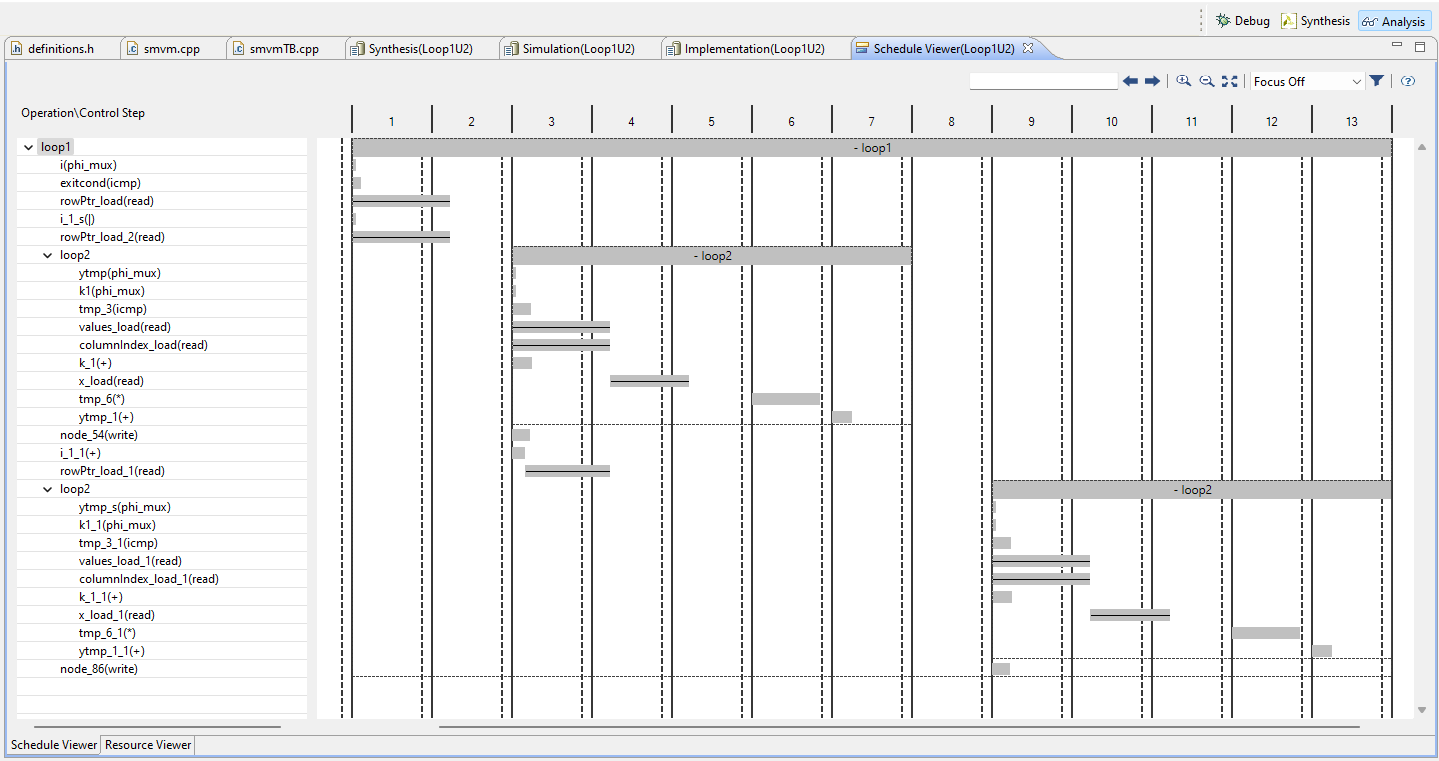
\includegraphics[width=1\textwidth]{solutions/s4/s4analysis.png}
	\caption{HLS Solution 4 Analysis}
\end{figure}

\begin{table}[h]
	\centering
	\begin{tabular}{|l|c|c|c|c|}
		\hline
		\textbf{Name}    & \textbf{BRAM\_18K} & \textbf{DSP48E} & \textbf{FF} & \textbf{LUT} \\ \hline
		DSP              & -                   & -               & -           & -            \\ 
		Expression       & -                   & 3               & 0           & 235          \\ 
		FIFO             & -                   & -               & -           & -            \\ 
		Instance         & -                   & -               & -           & -            \\ 
		Memory           & 0                   & -               & -          & -            \\ 
		Multiplexer      & -                   & -               & -           & 197          \\ 
		Register         & -                   & -               & 376         & -            \\ \hline
		\textbf{Total}   & 0                   & 3               & 376         & 432          \\ \hline
		\textbf{Available} & 280               & 220             & 106400      & 53200        \\ \hline
		\textbf{Utilization (\%)} & 0            & 1               & $\sim$0     & $\sim$0      \\ \hline
	\end{tabular}
	\caption{HLS Solution 4 Utilization Estimates Summary}
	\label{tab:hls-solution-4-utilization-estimates-summary}
\end{table}

Successivamente effettuando la C/RTL Cosimulation e l'Export RTL è possibile evidenziare i seguenti report.

\begin{table}[H]
	\centering
	\begin{tabular}{|c|c|c|c|c|c|c|c|}
		\hline
		\multicolumn{1}{|c|}{RTL} & \multicolumn{1}{|c|}{Status} & \multicolumn{3}{c|}{\textbf{Latency}} & \multicolumn{3}{c|}{\textbf{Interval}} \\
		&  & min & avg & max & min & avg & max \\
		\hline
		VHDL & Pass & 56 & 56 & 56 & NA & NA & NA \\
		\hline
	\end{tabular}
	\caption{HLS Solution 1 with Trip Count C/RTL Cosimulation Summary }
	\label{tab:hls-solution-1-cosimulation-summary}
\end{table}

\begin{table}[H]
	\centering
	\begin{minipage}[t]{0.45\linewidth}
		\centering
		\begin{tabular}{|l|r|}
			\hline
			\textbf{Resource} & \textbf{VHDL} \\
			\hline
			SLICE & 83 \\
			\hline
			LUT & 186 \\
			\hline
			FF & 292 \\
			\hline
			DSP & 3 \\
			\hline
			BRAM & 0 \\
			\hline
			SRL & 0 \\
			\hline
		\end{tabular}
		\caption{HLS Solution 2t Export RTL Resource Usage}
		\label{tab:hls-solution-2-export-rtl-resoruce-usage}
	\end{minipage}
	\hfill
	\begin{minipage}[t]{0.45\linewidth}
		\centering
		\begin{tabular}{|l|r|}
			\hline
			\textbf{Timing} & \textbf{VHDL} \\
			\hline
			CP required & 10.000 \\
			\hline
			CP achieved post-synthesis & 5.745 \\
			\hline
			CP achieved post-implementation & 5.692 \\
			\hline
		\end{tabular}
		\caption{HLS Solution 2 Export RTL Final Timing}
		\label{tab:hls-solution-2-export-rtl-final-timing}
	\end{minipage}
\end{table}